\documentclass{article}
\usepackage[utf8]{inputenc}
\usepackage{verbatim}
\usepackage{hyperref}
\usepackage{algorithm}
\usepackage[noend]{algpseudocode}
% \usepackage{titlesec}
\usepackage{amsmath}
\usepackage{graphicx}
\hypersetup{
  colorlinks=true,
  urlcolor=black,      % color of file links
  }
\usepackage{listings}% http://ctan.org/pkg/listings
\lstset{
  basicstyle=\ttfamily,
  mathescape
}
\usepackage{changepage}
\usepackage{tabularx}
\usepackage{setspace}
\usepackage{url}
\usepackage{multicol}
\usepackage{sectsty}

\newenvironment{indentsection}[1]%
{\begin{list}{}%
    {\setlength{\leftmargin}{#1}}%
    \item[]%
}
{\end{list}}

\newenvironment{unindentsection}[1]%
{\begin{list}{}%
    {\setlength{\leftmargin}{-0.5#1}}%
    \item[]%
}
{\end{list}}

% % format two pieces of text, one left aligned and one right aligned
\newcommand{\headerrow}[2]
{\begin{tabular*}{\linewidth}{l@{\extracolsep{\fill}}r}
    #1 &
    #2 \\
\end{tabular*}}

% %edit the section font and style
\sectionfont{\normalfont\sectionrule{0pt}{0pt}{-4pt}{1pt}}

% %make all sections cap and first letter capital
\newcommand{\tmpsection}[1]{}
\let\tmpsection=\section
% \renewcommand{\section}[1]{\tmpsection*{\textsc{#1}}}

% % set the line spacing
\setstretch{1.20}


\title{Flocking Bird Simulation\\
\large Indian Institute of Technology Delhi}
\author{Anubhav Palway (2016CS10368) \& Sunil Kumar (2016CS10314) }
\date{April 2018}

\begin{document}

\tableofcontents

\maketitle

\section{Abstract}
Here we will present the simulation of flocking behavior of the starling birds and their behavior when they are attacked by some predator. The first flocking-behaviour simulation was done by Craig Reynolds and he called his simulation program "Boids". It's still to this day the most used model for simulating flocking behaviour. We will also use this model to make simulation model. We will also look at flocking behavior of the birds when threatened by a group of predators. A set of forces are set up to describe the state of the prey, that in turn determines their behaviour in different scenarios. An effective strategy is found so all members of the flock can survive the predator attack, taking into account the advantages of the predator’s greater translational velocity and the prey’s higher angular velocity.

\section{Introduction}
The first flocking-behaviour simulation was done by Craig Reynolds in 1986 and he called his simulation program: "Boids"[1]. Boids was named after the simple agents in the system which he also called boids. The boids used a set of simple rules to determine how they would move. The three rules formatted by Reynolds in his Boids program are still the basis of modern flocking simulation and are widely used to these days. These are the three rules as they are described by Reynolds:\\
\begin{itemize}
    \item \textbf{Separation: } Steer to avoid crowding local flocking.
    \item \textbf{Alignment: } Steer towards the average heading of local flockmate.
    \item \textbf{Cohesion: } Steer to move toward the average position of local flockmates.
    
\end{itemize}

\bigbreak
In the subsequent sections, we will describe the basic terminology used and, the algorithms used to satisfy the three properties of the Reynolds model. Then we will introduce the saturation functions (for the range of velocities of the boids), unicycle model (used for calculating the velocities), energy constraints and the various forces which we consider for the simulation purposes and the mathematics behind it.

\section{Defintions}

\subsection{Boid}
A representation of a bird in flocking simulations. The word is most commonly used in the context of Boids, the original computer simulation of flocking behaviour by Craig Reynolds and derivative of Boids. The name "boid" corresponds to a shortened version of "bird-oid object", which refers to a bird-like object.

\subsection{Flocking Behaviour}
Flocking behavior is the behavior exhibited when a group of birds, called a flock, are foraging or in flight. There are parallels with the shoaling behavior of fish, the swarming behavior of insects, and herd behavior of land animals.Computer simulations and mathematical models which have been developed to emulate the flocking behaviors of birds can generally be applied also to the "flocking" behavior of other species. As a result, the term "flocking" is sometimes applied, in computer science, to species other than birds.

\subsection{Emergent Behaviour}
When individual objects interact with each other directly or indirectly to create much more complex results. Another characteristic of emergent behaviour is that the end result is hard to predict even if each interaction in itself is simplistic. Anthills, economics, the evolution are all examples of how agents abiding to relatively simple rules can create a system more complex than the sum of its parts. Reynolds Boids algorithm can be said to create an emergent behaviour.

\section{Algorithm}

\subsection{An overview}
This model follows this simple structure: calculate the current state, draw the state on the screen and repeat Algorithm 1 shows the structure of a typical Boids implementation. The three rules of the Boids algorithm only changes the speed and course of the boid and can be applied in any order. After the velocity has been updated, we can update the positions of the boids. We update the position by simply calculating where it would be if it fly straight for some small amount of time.

\begin{algorithm}
\caption{An overview}\label{euclid}
\begin{algorithmic}[1]
\State $\textit{Data:   } \text{A group of boids.}$
\State $\textit{Result:   } \text{Simulates flocking behaviour with an animation.}$

\ForAll {Frame}
    \ForAll{Boid} 
    \State $\text{separation(boid);} $
    \State $\text{cohesion(boid);} $
    \State $\text{alignment(boid);} $
    \EndFor
    \ForAll{Boid} 
    \State $boid.x \gets cos(boid.course(\theta)) * b.velocity * dTime $
    \State $boid.y \gets sin(boid.course(\theta)) * cos(boid.course(\phi)) * b.velocity * dTime $
    \State $boid.z \gets sin(boid.course(\theta)) * sin(boid.course(\phi)) * b.velocity * dTime $
    \State $\text{draw(boid)} $
    \EndFor
\Endfor

\end{algorithmic}

\end{algorithm}

\subsection{Boid}
The boid is the bird representation in flocking simulation model. Each boid object should at least have the following attributes to describe the state it is in.

\begin{itemize}
    \item \textbf{Loaction: } The x, y and z coordinates of the current position of the boid.
    \item \textbf{Course: } The angle of the current course course of the boid.
    \item \textbf{Veclocity: } The speed of which the boid is traveling.
\end{itemize}
\bigbreak
The course and speed could of course be represented by a equivalent velocity vector instead. But often more attributes is needed to make the simulation more convincing. Putting an upper limit on how fast the boids can move and turn is a common improvement.

\subsection{Cohesion}

Steer to move toward the average position of local flockmates.[2] Cohesion is the rule that keeps the flock together, without it there would not be any flocking at all. Algorithm 2 shows how this algorithm could be implemented, it finds the average position of the neighbourhood boids and tries to move the boid towards it.\\

\begin{center}
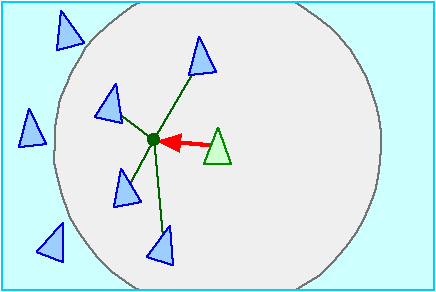
\includegraphics[scale=0.4]{cohesion.png} 
\end{center}

\begin{algorithm}
\caption{First Rule: Cohesion}\label{euclid}
\begin{algorithmic}[1]
\State $\textit{Data:   } \text{A boid.}$
\State $\textit{Result:   } \text{The course of the boid is updated}$
\\
\State $\text{goal} \gets \text{(0,0);}$
\State $\text{neighbours} \gets \text{getNeighbours(boid);}$

\ForAll {nBoid in neighbours}
    \State $ goal \gets goals + positionOf(nBoid)$
\Endfor
\State $\text{goal} \gets \text{goal / neighbours.size()}$
\State $\text{steerToward(goal,boid)}$
\end{algorithmic}

\end{algorithm}

\subsection{Separation}

Steer to avoid crowding local flockmates.[3] If a flocking behaviour is to be convincing it must also avoid collisions between the boids. This rule attempts steer the boid away from possible collisions. It's important to note that the distance from which the boids start to avoid each other must be less than the distance from each other(due to the cohesion rule). Otherwise no flocks would be formed.\\

\begin{center}
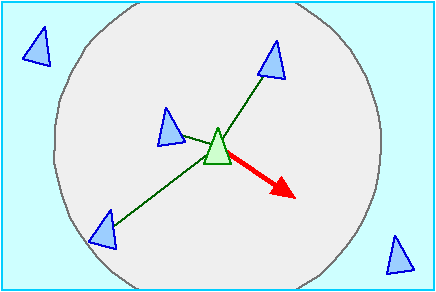
\includegraphics[scale=0.4]{separation.png} 
\end{center}

\begin{algorithm}
\caption{Second Rule: Separation}\label{euclid}
\begin{algorithmic}[1]
\State $\textit{Data:   } \text{A boid.}$
\State $\textit{Result:   } \text{The course of the boid is updated}$
\\
\State $\text{goal} \gets \text{(0,0);}$
\State $\text{neighbours} \gets \text{getNeighbours(boid);}$

\ForAll {nBoid in neighbours}
    \State $ goal \gets goals + positionOf(Boid) - positionOf(nBoid);$
\Endfor
\State $\text{goal} \gets \text{goal / neighbours.size()}$
\State $\text{steerToward(goal,boid)}$
\end{algorithmic}

\end{algorithm}

\subsection{Alignment}

Steer towards the average heading of local flockmates.[3] This rule tries to make the boids mimic each other's course and speed. If this rule was not used the boids would bounce around a lot and not form the beautiful flocking patterns that can be seen in real flocks.\\

\begin{center}
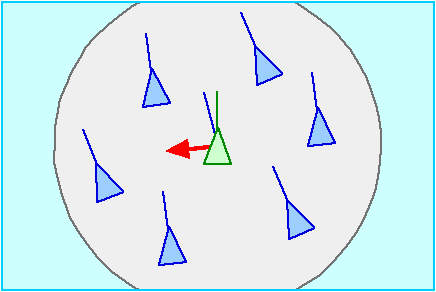
\includegraphics[scale=0.4]{alignment.png} 
\end{center}

\begin{algorithm}
\caption{Third Rule: Alignment}\label{euclid}
\begin{algorithmic}[1]
\State $\textit{Data:   } \text{A boid.}$
\State $\textit{Result:   } \text{The course and velocity of the boid is updated}$
\\
\State $\text{dCourse} \gets \text{0;}$
\State $\text{dVelocity} \gets \text{0;}$
\State $\text{neighbours} \gets \text{getNeighbours(boid);}$

\ForAll {nBoid in neighbours}
    \State $ dCourse \gets dCourse + getCourse(nBoid) - getCourse(Boid);$
    \State $ dVelocity \gets dVelocity + getVelocity(nBoid) - getVelocity(Boid);$
\Endfor
\State $\text{dCourse} \gets \text{dCourse / neighbours.size()}$
\State $\text{dVelocity} \gets \text{dVelocity / neighbours.size()}$
\State $\text{boid.addCourse(dCourse)}$
\State $\text{boid.addVelocity(dVelocity)}$
\end{algorithmic}

\end{algorithm}

\pagebreak
\subsection{Defining the neighbourhood}
The neighbourhood of a boid is the neighbourhood it perceives and is a core part of this algorithm. The neighbourhood decides what other boids, a boid should take into account when deciding the next move.
Each pseudo code of the three rules of the Boids algorithm (algorithms 2, 3
and 4) uses a function called getNeighbours(Boid) to get the neighbors of the given
boid. The three rules could and should use different implementation of the get-
Neighbours(Boid) method. It’s important for example that the separation rule only
acts on the closest boids. If separation and cohesion would work on the same neigh-
bourhood they would cancel each other out.
Raynolds original implementation simply defined the neighbors as the boids
within a certain radius. Another possible definition of the neighbourhood is to let
each boid look at the N closest boids instead. This thesis attempts to compare the
two definitions to find strengths and weaknesses in both definitions and find under
what circumstances either is superior.\\

\begin{center}
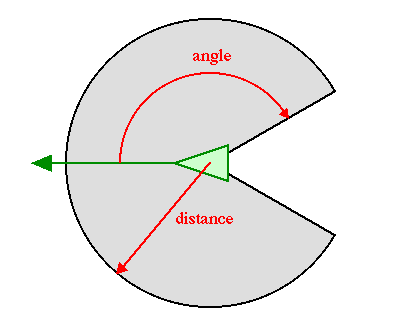
\includegraphics[scale=0.4]{neighbour.png} 
\end{center}

\section{Mathematics}

\subsection{Velocity Function}
The velocities in different can be formulated as a time dependent equation system:\\
\begin{equation}
    \begin{cases}
    \Dot{x} = v \cdot cos\theta \\
    \Dot{y} = v \cdot sin\theta \cdot cos \phi\\
    \Dot{z} = v \cdot sin\theta \cdot sin \phi\\
    \Dot{\theta} = \omega
    \end{cases}
\end{equation}

\subsection{Saturation Function}
Since there is an upper and lower limit for the discussed velocities, we have to limit those. It is done with the help of a saturation function.\\
The saturation function for the translational velocity is given by:\\
\begin{equation}
    sat(v)=\begin{cases}
    v_{max}  & $\text{if $v>v_{max}$}$\\
    v  & $\text{if $0<v<v_{max}$}$\\
    0  & $\text{if $v<0$}$
    \end{cases}
\end{equation}

where $v_{max}$ is the boid's maximum velocity.\\

Similarly, saturation function for angular velocity is:\\
\begin{equation}
    sat(\omega)=\begin{cases}
    \omega _{max}  & $\text{if $\omega>\omega _{max}$}$\\
    \omega  & $\text{if $-\omega _{max}<\omega<\omega _{max}$}$\\
    -\omega _{max}  & $\text{if $\omega<-\omega _{max}$}$
    \end{cases}
\end{equation}
where $\omega _{max}$ is the boid's maximum velocity.\\

\section{Energy Constraint}
An energy constraint, is needed in the model to make it realistic as the birds cannot run for an infinite amount of time. This contraint also makes the bird's movement finite, because when energy becomes zero, all the forces turn to zero. The formula for this is defined as:
\begin{equation}
E _{i} (t) = E _{i,0} - c _{E} \cdot \int_{0}^{t _{1}} v _{i} (t)^2 dt   
\end{equation}
where E _{i,0} is the bird's initial velocity, c_{E} is a constant that is related to bird's mass and v _{i}(t) is the translational velocity of agent i at time t which lies in the interval [0,t_{1}] where t_{1} is the length of the simulation. Assumption made here is that the energy consumption is directly proportional to the square of the translational velocity of the bird.

\section{Different forces to consider}

\subsection{Flocking Force}
For the flock to stay together, there is a force needed to hold the birds together. 
This is done by taking the position of the agent's center of mass,  and have an attractive force acting towards it. This forces is the reason for flocking (see fig). This force is a weak force and only acts when birds sense no danger.
\begin{equation}
    {f_{i,fl}} = c_{fl} \cdot ({z_{mc}-z_{i}})
\end{equation}
\begin{equation}
    z_{mc}=\sum_{i=0}^{n}\dfrac{z_{i}}{n}
\end{equation}
where cfl is the overall magnitude of the force.\\ \\ 
\begin{center}
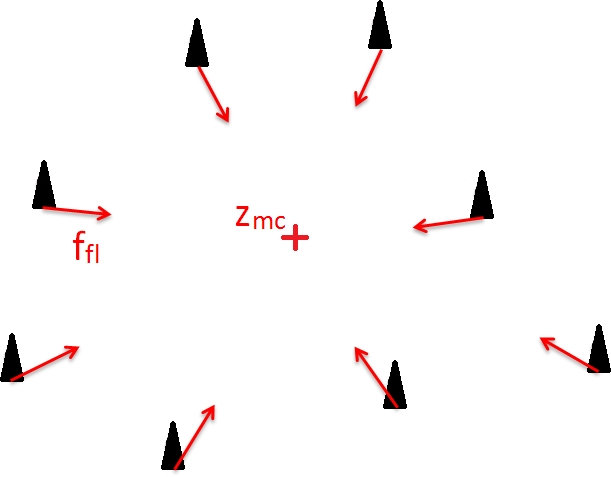
\includegraphics[scale=0.4]{fig9.png} 
\end{center}



\subsection{Predator Avoidance Force}
The flocking behaviour is affected when an bird faces danger, in our case;
caused by a predator. The members senses the presence of the predator. If the predator is closer than the predator detection distance i.e., Rd then only this force comes into act (see fig) .The most effective strategy to avoid predators was found to be the following equation which takes all attacking predators, pk into account:
\begin{equation}
    f_{i,pa} = \sum_{k:|{z_{i}-p_{k}}|<R_{d}}^{} c_{pa} \cdot \dfrac{1}{1+\exp{\omega_{pa}(|{z_{i}-p_{k})-R_{pa}} + 0.3
\end{equation}

where c_{pa} and \omega _{pa} gives the force's magnitude and gradient respectively.
\begin{center}
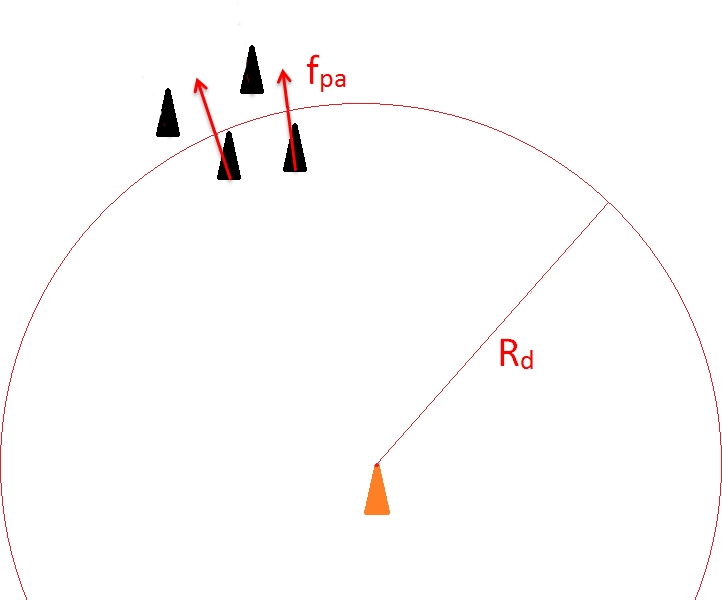
\includegraphics[scale=0.4]{fig3.png} 
\end{center}

\pagebreak

\section{Refereces}
1) Craig W. Reynolds. Flocks, herds, and schools: A distributed behavioral model. In Computer Graphics, pages 25–34, 1987.\\
2) Craig W. Reynolds. Boids, Background and Update . http://www.red3d.com/ cwr/boids/, 2007. [Online; accessed 14-April-2011]. \\
3) \href{http://www.red3d.com/cwr/steer/gdc99/}{http://www.red3d.com/cwr/steer/gdc99/}\\
4) \href{http://cp3-origins.dk/a/14187}{http://cp3-origins.dk/a/14187}\\
5) \href{https://en.wikipedia.org/wiki/Flocking_(behavior)}{https://en.wikipedia.org/wiki/Flocking_(behavior)}\\
6) \href{https://en.wikipedia.org/wiki/Boids}{https://en.wikipedia.org/wiki/Boids}\\
7) \href{http://www.csc.kth.se/utbildning/kandidatexjobb/datateknik/2011/rapport/erneholm_carl-oscar_K11044.pdf}{http://www.csc.kth.se/utbildning/kandidatexjobb/datateknik/2011/rapport/erneholm_carl-oscar_K11044.pdf}

\end{document}
